\documentclass[twoside]{book}

% Packages required by doxygen
\usepackage{fixltx2e}
\usepackage{calc}
\usepackage{doxygen}
\usepackage[export]{adjustbox} % also loads graphicx
\usepackage{graphicx}
\usepackage[utf8]{inputenc}
\usepackage{makeidx}
\usepackage{multicol}
\usepackage{multirow}
\PassOptionsToPackage{warn}{textcomp}
\usepackage{textcomp}
\usepackage[nointegrals]{wasysym}
\usepackage[table]{xcolor}

% Font selection
\usepackage[T1]{fontenc}
\usepackage[scaled=.90]{helvet}
\usepackage{courier}
\usepackage{amssymb}
\usepackage{sectsty}
\renewcommand{\familydefault}{\sfdefault}
\allsectionsfont{%
  \fontseries{bc}\selectfont%
  \color{darkgray}%
}
\renewcommand{\DoxyLabelFont}{%
  \fontseries{bc}\selectfont%
  \color{darkgray}%
}
\newcommand{\+}{\discretionary{\mbox{\scriptsize$\hookleftarrow$}}{}{}}

% Page & text layout
\usepackage{geometry}
\geometry{%
  a4paper,%
  top=2.5cm,%
  bottom=2.5cm,%
  left=2.5cm,%
  right=2.5cm%
}
\tolerance=750
\hfuzz=15pt
\hbadness=750
\setlength{\emergencystretch}{15pt}
\setlength{\parindent}{0cm}
\setlength{\parskip}{3ex plus 2ex minus 2ex}
\makeatletter
\renewcommand{\paragraph}{%
  \@startsection{paragraph}{4}{0ex}{-1.0ex}{1.0ex}{%
    \normalfont\normalsize\bfseries\SS@parafont%
  }%
}
\renewcommand{\subparagraph}{%
  \@startsection{subparagraph}{5}{0ex}{-1.0ex}{1.0ex}{%
    \normalfont\normalsize\bfseries\SS@subparafont%
  }%
}
\makeatother

% Headers & footers
\usepackage{fancyhdr}
\pagestyle{fancyplain}
\fancyhead[LE]{\fancyplain{}{\bfseries\thepage}}
\fancyhead[CE]{\fancyplain{}{}}
\fancyhead[RE]{\fancyplain{}{\bfseries\leftmark}}
\fancyhead[LO]{\fancyplain{}{\bfseries\rightmark}}
\fancyhead[CO]{\fancyplain{}{}}
\fancyhead[RO]{\fancyplain{}{\bfseries\thepage}}
\fancyfoot[LE]{\fancyplain{}{}}
\fancyfoot[CE]{\fancyplain{}{}}
\fancyfoot[RE]{\fancyplain{}{\bfseries\scriptsize Generated by Doxygen }}
\fancyfoot[LO]{\fancyplain{}{\bfseries\scriptsize Generated by Doxygen }}
\fancyfoot[CO]{\fancyplain{}{}}
\fancyfoot[RO]{\fancyplain{}{}}
\renewcommand{\footrulewidth}{0.4pt}
\renewcommand{\chaptermark}[1]{%
  \markboth{#1}{}%
}
\renewcommand{\sectionmark}[1]{%
  \markright{\thesection\ #1}%
}

% Indices & bibliography
\usepackage{natbib}
\usepackage[titles]{tocloft}
\setcounter{tocdepth}{3}
\setcounter{secnumdepth}{5}
\makeindex

% Hyperlinks (required, but should be loaded last)
\usepackage{ifpdf}
\ifpdf
  \usepackage[pdftex,pagebackref=true]{hyperref}
\else
  \usepackage[ps2pdf,pagebackref=true]{hyperref}
\fi
\hypersetup{%
  colorlinks=true,%
  linkcolor=blue,%
  citecolor=blue,%
  unicode%
}

% Custom commands
\newcommand{\clearemptydoublepage}{%
  \newpage{\pagestyle{empty}\cleardoublepage}%
}

\usepackage{caption}
\captionsetup{labelsep=space,justification=centering,font={bf},singlelinecheck=off,skip=4pt,position=top}

%===== C O N T E N T S =====

\begin{document}

% Titlepage & ToC
\hypersetup{pageanchor=false,
             bookmarksnumbered=true,
             pdfencoding=unicode
            }
\pagenumbering{alph}
\begin{titlepage}
\vspace*{7cm}
\begin{center}%
{\Large Human Obstacle Detector and Tracker }\\
\vspace*{1cm}
{\large Generated by Doxygen 1.8.13}\\
\end{center}
\end{titlepage}
\clearemptydoublepage
\pagenumbering{roman}
\tableofcontents
\clearemptydoublepage
\pagenumbering{arabic}
\hypersetup{pageanchor=true}

%--- Begin generated contents ---
\chapter{File Index}
\section{File List}
Here is a list of all documented files with brief descriptions\+:\begin{DoxyCompactList}
\item\contentsline{section}{src/\hyperlink{action__server__node_8cpp}{action\+\_\+server\+\_\+node.\+cpp} \\*R\+OS node to spin the Task\+Action\+Server up }{\pageref{action__server__node_8cpp}}{}
\item\contentsline{section}{src/\hyperlink{arm__controller_8cpp}{arm\+\_\+controller.\+cpp} \\*Defining the class to control the arm movement of the robot }{\pageref{arm__controller_8cpp}}{}
\item\contentsline{section}{src/\hyperlink{gripper__controller_8cpp}{gripper\+\_\+controller.\+cpp} \\*Defining the class to control the gripper movement of the robot }{\pageref{gripper__controller_8cpp}}{}
\item\contentsline{section}{src/\hyperlink{head__controller_8cpp}{head\+\_\+controller.\+cpp} \\*Defining the class to control the head movement of the robot }{\pageref{head__controller_8cpp}}{}
\item\contentsline{section}{src/\hyperlink{map__navigator_8cpp}{map\+\_\+navigator.\+cpp} \\*Definitions of Map\+Navigator class }{\pageref{map__navigator_8cpp}}{}
\item\contentsline{section}{src/\hyperlink{movebaseaction__wrapper_8cpp}{movebaseaction\+\_\+wrapper.\+cpp} \\*Definitions of Move\+Base\+Action\+Wrapper class }{\pageref{movebaseaction__wrapper_8cpp}}{}
\item\contentsline{section}{src/\hyperlink{pick__place__controller_8cpp}{pick\+\_\+place\+\_\+controller.\+cpp} \\*Defining the class to control all the pick and place tasks to be performed by the robot }{\pageref{pick__place__controller_8cpp}}{}
\item\contentsline{section}{src/\hyperlink{robot__controller_8cpp}{robot\+\_\+controller.\+cpp} \\*Defining the class to control all the different joint movements of the robot }{\pageref{robot__controller_8cpp}}{}
\item\contentsline{section}{src/\hyperlink{task__action__client_8cpp}{task\+\_\+action\+\_\+client.\+cpp} \\*Definitions of Task\+Action\+Client class }{\pageref{task__action__client_8cpp}}{}
\item\contentsline{section}{src/\hyperlink{task__action__server_8cpp}{task\+\_\+action\+\_\+server.\+cpp} \\*Definitions of Task\+Action\+Server class }{\pageref{task__action__server_8cpp}}{}
\item\contentsline{section}{src/\hyperlink{task__publisher_8cpp}{task\+\_\+publisher.\+cpp} \\*Definitions of Task\+Publisher class }{\pageref{task__publisher_8cpp}}{}
\item\contentsline{section}{src/\hyperlink{task__subscriber__node_8cpp}{task\+\_\+subscriber\+\_\+node.\+cpp} \\*R\+OS node to spawn the subscriber of the task topic }{\pageref{task__subscriber__node_8cpp}}{}
\item\contentsline{section}{src/\hyperlink{torso__controller_8cpp}{torso\+\_\+controller.\+cpp} \\*Defining the class to control the torso movement of the robot }{\pageref{torso__controller_8cpp}}{}
\item\contentsline{section}{src/\hyperlink{user__interface__node_8cpp}{user\+\_\+interface\+\_\+node.\+cpp} \\*R\+OS node for to spawn user interface and have some interaction with the user over command line }{\pageref{user__interface__node_8cpp}}{}
\item\contentsline{section}{test/\hyperlink{main_8cpp}{main.\+cpp} \\*Main for controller tests }{\pageref{main_8cpp}}{}
\item\contentsline{section}{test/\hyperlink{test__arm__controller_8cpp}{test\+\_\+arm\+\_\+controller.\+cpp} \\*Testing of Arm\+Controller class }{\pageref{test__arm__controller_8cpp}}{}
\item\contentsline{section}{test/\hyperlink{test__aruco__detector_8cpp}{test\+\_\+aruco\+\_\+detector.\+cpp} \\*Testing of Aruco\+Detector class }{\pageref{test__aruco__detector_8cpp}}{}
\item\contentsline{section}{test/\hyperlink{test__gripper__controller_8cpp}{test\+\_\+gripper\+\_\+controller.\+cpp} \\*Testing of Gripper\+Controller class }{\pageref{test__gripper__controller_8cpp}}{}
\item\contentsline{section}{test/\hyperlink{test__head__controller_8cpp}{test\+\_\+head\+\_\+controller.\+cpp} \\*Testing of Head\+Controller class }{\pageref{test__head__controller_8cpp}}{}
\item\contentsline{section}{test/\hyperlink{test__map__navigator_8cpp}{test\+\_\+map\+\_\+navigator.\+cpp} \\*Testing of Map\+Navigator class }{\pageref{test__map__navigator_8cpp}}{}
\item\contentsline{section}{test/\hyperlink{test__movebaseaction__wrapper_8cpp}{test\+\_\+movebaseaction\+\_\+wrapper.\+cpp} \\*Testing of Move\+Base\+Action\+Wrapper class }{\pageref{test__movebaseaction__wrapper_8cpp}}{}
\item\contentsline{section}{test/\hyperlink{test__pick__place__controller_8cpp}{test\+\_\+pick\+\_\+place\+\_\+controller.\+cpp} \\*Testing of Pick\+Place\+Controller class }{\pageref{test__pick__place__controller_8cpp}}{}
\item\contentsline{section}{test/\hyperlink{test__task__action_8cpp}{test\+\_\+task\+\_\+action.\+cpp} \\*Testing of Guidance\+Task and Delivery\+Task class }{\pageref{test__task__action_8cpp}}{}
\item\contentsline{section}{test/\hyperlink{test__torso__controller_8cpp}{test\+\_\+torso\+\_\+controller.\+cpp} \\*Testing of Torso\+Controller class }{\pageref{test__torso__controller_8cpp}}{}
\end{DoxyCompactList}

\chapter{File Documentation}
\hypertarget{map__navigator_8cpp}{}\doxysection{src/map\+\_\+navigator.cpp File Reference}
\label{map__navigator_8cpp}\index{src/map\_navigator.cpp@{src/map\_navigator.cpp}}


Definitions of Map\+Navigator class.  


{\ttfamily \#include $<$nurse-\/bot/map\+\_\+navigator.\+hpp$>$}\newline
Include dependency graph for map\+\_\+navigator.\+cpp\+:
\nopagebreak
\begin{figure}[H]
\begin{center}
\leavevmode
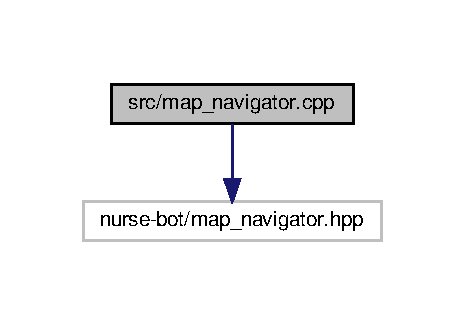
\includegraphics[width=241pt]{map__navigator_8cpp__incl}
\end{center}
\end{figure}


\doxysubsection{Detailed Description}
Definitions of Map\+Navigator class. 

M\+IT License

Copyright (c) 2021 Sakshi Kakde, Siddharth Telang, Anubhav Paras

Permission is hereby granted, free of charge, to any person obtaining a copy of this software and associated documentation files (the \char`\"{}\+Software\char`\"{}), to deal in the Software without restriction, including without limitation the rights to use, copy, modify, merge, publish, distribute, sublicense, and/or sell copies of the Software, and to permit persons to whom the Software is furnished to do so, subject to the following conditions\+:

The above copyright notice and this permission notice shall be included in all copies or substantial portions of the Software.

T\+HE S\+O\+F\+T\+W\+A\+RE IS P\+R\+O\+V\+I\+D\+ED \char`\"{}\+A\+S I\+S\char`\"{}, W\+I\+T\+H\+O\+UT W\+A\+R\+R\+A\+N\+TY OF A\+NY K\+I\+ND, E\+X\+P\+R\+E\+SS OR I\+M\+P\+L\+I\+ED, I\+N\+C\+L\+U\+D\+I\+NG B\+UT N\+OT L\+I\+M\+I\+T\+ED TO T\+HE W\+A\+R\+R\+A\+N\+T\+I\+ES OF M\+E\+R\+C\+H\+A\+N\+T\+A\+B\+I\+L\+I\+TY, F\+I\+T\+N\+E\+SS F\+OR A P\+A\+R\+T\+I\+C\+U\+L\+AR P\+U\+R\+P\+O\+SE A\+ND N\+O\+N\+I\+N\+F\+R\+I\+N\+G\+E\+M\+E\+NT. IN NO E\+V\+E\+NT S\+H\+A\+LL T\+HE A\+U\+T\+H\+O\+RS OR C\+O\+P\+Y\+R\+I\+G\+HT H\+O\+L\+D\+E\+RS BE L\+I\+A\+B\+LE F\+OR A\+NY C\+L\+A\+IM, D\+A\+M\+A\+G\+ES OR O\+T\+H\+ER L\+I\+A\+B\+I\+L\+I\+TY, W\+H\+E\+T\+H\+ER IN AN A\+C\+T\+I\+ON OF C\+O\+N\+T\+R\+A\+CT, T\+O\+RT OR O\+T\+H\+E\+R\+W\+I\+SE, A\+R\+I\+S\+I\+NG F\+R\+OM, O\+UT OF OR IN C\+O\+N\+N\+E\+C\+T\+I\+ON W\+I\+TH T\+HE S\+O\+F\+T\+W\+A\+RE OR T\+HE U\+SE OR O\+T\+H\+ER D\+E\+A\+L\+I\+N\+GS IN T\+HE S\+O\+F\+T\+W\+A\+RE.

\begin{DoxyAuthor}{Author}
Sakshi Kakde (\href{mailto:sakshi@umd.edu}{\texttt{ sakshi@umd.\+edu}}) 

Siddharth Telang (\href{mailto:stelang@umd.edu}{\texttt{ stelang@umd.\+edu}}) 

Anubhav Paras (\href{mailto:anubhavp@umd.edu}{\texttt{ anubhavp@umd.\+edu}}) 
\end{DoxyAuthor}
\begin{DoxyVersion}{Version}
0.\+1 
\end{DoxyVersion}
\begin{DoxyDate}{Date}
2021-\/11-\/27
\end{DoxyDate}
\begin{DoxyCopyright}{Copyright}
Copyright (c) 2021 
\end{DoxyCopyright}

\hypertarget{movebaseaction__wrapper_8cpp}{}\section{src/movebaseaction\+\_\+wrapper.cpp File Reference}
\label{movebaseaction__wrapper_8cpp}\index{src/movebaseaction\+\_\+wrapper.\+cpp@{src/movebaseaction\+\_\+wrapper.\+cpp}}


Definitions of Move\+Base\+Action\+Wrapper class.  


{\ttfamily \#include $<$nurse-\/bot/movebaseaction\+\_\+wrapper.\+hpp$>$}\newline
{\ttfamily \#include $<$memory$>$}\newline
Include dependency graph for movebaseaction\+\_\+wrapper.\+cpp\+:
\nopagebreak
\begin{figure}[H]
\begin{center}
\leavevmode
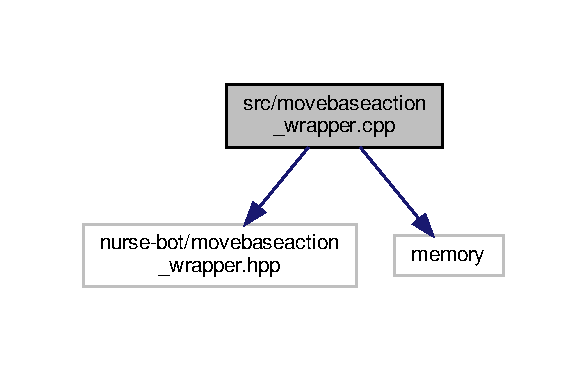
\includegraphics[width=282pt]{movebaseaction__wrapper_8cpp__incl}
\end{center}
\end{figure}


\subsection{Detailed Description}
Definitions of Move\+Base\+Action\+Wrapper class. 

M\+IT License

Copyright (c) 2021 Sakshi Kakde, Siddharth Telang, Anubhav Paras

Permission is hereby granted, free of charge, to any person obtaining a copy of this software and associated documentation files (the \char`\"{}\+Software\char`\"{}), to deal in the Software without restriction, including without limitation the rights to use, copy, modify, merge, publish, distribute, sublicense, and/or sell copies of the Software, and to permit persons to whom the Software is furnished to do so, subject to the following conditions\+:

The above copyright notice and this permission notice shall be included in all copies or substantial portions of the Software.

T\+HE S\+O\+F\+T\+W\+A\+RE IS P\+R\+O\+V\+I\+D\+ED \char`\"{}\+A\+S I\+S\char`\"{}, W\+I\+T\+H\+O\+UT W\+A\+R\+R\+A\+N\+TY OF A\+NY K\+I\+ND, E\+X\+P\+R\+E\+SS OR I\+M\+P\+L\+I\+ED, I\+N\+C\+L\+U\+D\+I\+NG B\+UT N\+OT L\+I\+M\+I\+T\+ED TO T\+HE W\+A\+R\+R\+A\+N\+T\+I\+ES OF M\+E\+R\+C\+H\+A\+N\+T\+A\+B\+I\+L\+I\+TY, F\+I\+T\+N\+E\+SS F\+OR A P\+A\+R\+T\+I\+C\+U\+L\+AR P\+U\+R\+P\+O\+SE A\+ND N\+O\+N\+I\+N\+F\+R\+I\+N\+G\+E\+M\+E\+NT. IN NO E\+V\+E\+NT S\+H\+A\+LL T\+HE A\+U\+T\+H\+O\+RS OR C\+O\+P\+Y\+R\+I\+G\+HT H\+O\+L\+D\+E\+RS BE L\+I\+A\+B\+LE F\+OR A\+NY C\+L\+A\+IM, D\+A\+M\+A\+G\+ES OR O\+T\+H\+ER L\+I\+A\+B\+I\+L\+I\+TY, W\+H\+E\+T\+H\+ER IN AN A\+C\+T\+I\+ON OF C\+O\+N\+T\+R\+A\+CT, T\+O\+RT OR O\+T\+H\+E\+R\+W\+I\+SE, A\+R\+I\+S\+I\+NG F\+R\+OM, O\+UT OF OR IN C\+O\+N\+N\+E\+C\+T\+I\+ON W\+I\+TH T\+HE S\+O\+F\+T\+W\+A\+RE OR T\+HE U\+SE OR O\+T\+H\+ER D\+E\+A\+L\+I\+N\+GS IN T\+HE S\+O\+F\+T\+W\+A\+RE.

\begin{DoxyAuthor}{Author}
Sakshi Kakde (\href{mailto:sakshi@umd.edu}{\tt sakshi@umd.\+edu}) 

Siddharth Telang (\href{mailto:stelang@umd.edu}{\tt stelang@umd.\+edu}) 

Anubhav Paras (\href{mailto:anubhavp@umd.edu}{\tt anubhavp@umd.\+edu}) 
\end{DoxyAuthor}
\begin{DoxyVersion}{Version}
0.\+1 
\end{DoxyVersion}
\begin{DoxyDate}{Date}
2021-\/11-\/27
\end{DoxyDate}
\begin{DoxyCopyright}{Copyright}
Copyright (c) 2021 
\end{DoxyCopyright}

\hypertarget{task__publisher_8cpp}{}\section{src/task\+\_\+publisher.cpp File Reference}
\label{task__publisher_8cpp}\index{src/task\+\_\+publisher.\+cpp@{src/task\+\_\+publisher.\+cpp}}


Definitions of Task\+Publisher class.  


{\ttfamily \#include $<$nurse\+\_\+bot/\+Task.\+h$>$}\newline
{\ttfamily \#include $<$nurse-\/bot/task\+\_\+publisher.\+hpp$>$}\newline
Include dependency graph for task\+\_\+publisher.\+cpp\+:
\nopagebreak
\begin{figure}[H]
\begin{center}
\leavevmode
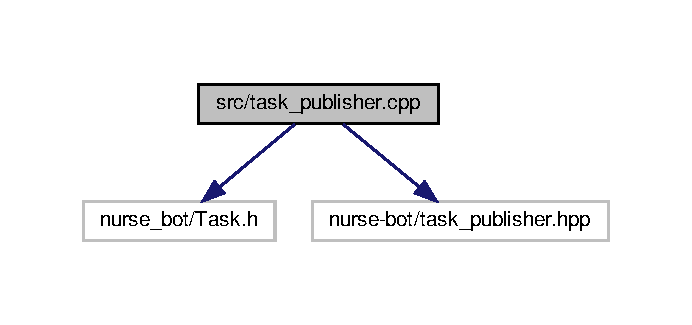
\includegraphics[width=332pt]{task__publisher_8cpp__incl}
\end{center}
\end{figure}


\subsection{Detailed Description}
Definitions of Task\+Publisher class. 

M\+IT License

Copyright (c) 2021 Sakshi Kakde, Siddharth Telang, Anubhav Paras

Permission is hereby granted, free of charge, to any person obtaining a copy of this software and associated documentation files (the \char`\"{}\+Software\char`\"{}), to deal in the Software without restriction, including without limitation the rights to use, copy, modify, merge, publish, distribute, sublicense, and/or sell copies of the Software, and to permit persons to whom the Software is furnished to do so, subject to the following conditions\+:

The above copyright notice and this permission notice shall be included in all copies or substantial portions of the Software.

T\+HE S\+O\+F\+T\+W\+A\+RE IS P\+R\+O\+V\+I\+D\+ED \char`\"{}\+A\+S I\+S\char`\"{}, W\+I\+T\+H\+O\+UT W\+A\+R\+R\+A\+N\+TY OF A\+NY K\+I\+ND, E\+X\+P\+R\+E\+SS OR I\+M\+P\+L\+I\+ED, I\+N\+C\+L\+U\+D\+I\+NG B\+UT N\+OT L\+I\+M\+I\+T\+ED TO T\+HE W\+A\+R\+R\+A\+N\+T\+I\+ES OF M\+E\+R\+C\+H\+A\+N\+T\+A\+B\+I\+L\+I\+TY, F\+I\+T\+N\+E\+SS F\+OR A P\+A\+R\+T\+I\+C\+U\+L\+AR P\+U\+R\+P\+O\+SE A\+ND N\+O\+N\+I\+N\+F\+R\+I\+N\+G\+E\+M\+E\+NT. IN NO E\+V\+E\+NT S\+H\+A\+LL T\+HE A\+U\+T\+H\+O\+RS OR C\+O\+P\+Y\+R\+I\+G\+HT H\+O\+L\+D\+E\+RS BE L\+I\+A\+B\+LE F\+OR A\+NY C\+L\+A\+IM, D\+A\+M\+A\+G\+ES OR O\+T\+H\+ER L\+I\+A\+B\+I\+L\+I\+TY, W\+H\+E\+T\+H\+ER IN AN A\+C\+T\+I\+ON OF C\+O\+N\+T\+R\+A\+CT, T\+O\+RT OR O\+T\+H\+E\+R\+W\+I\+SE, A\+R\+I\+S\+I\+NG F\+R\+OM, O\+UT OF OR IN C\+O\+N\+N\+E\+C\+T\+I\+ON W\+I\+TH T\+HE S\+O\+F\+T\+W\+A\+RE OR T\+HE U\+SE OR O\+T\+H\+ER D\+E\+A\+L\+I\+N\+GS IN T\+HE S\+O\+F\+T\+W\+A\+RE.

\begin{DoxyAuthor}{Author}
Sakshi Kakde (\href{mailto:sakshi@umd.edu}{\tt sakshi@umd.\+edu}) 

Siddharth Telang (\href{mailto:stelang@umd.edu}{\tt stelang@umd.\+edu}) 

Anubhav Paras (\href{mailto:anubhavp@umd.edu}{\tt anubhavp@umd.\+edu}) 
\end{DoxyAuthor}
\begin{DoxyVersion}{Version}
0.\+1 
\end{DoxyVersion}
\begin{DoxyDate}{Date}
2021-\/11-\/27
\end{DoxyDate}
\begin{DoxyCopyright}{Copyright}
Copyright (c) 2021 
\end{DoxyCopyright}

\hypertarget{task__subscriber__node_8cpp}{}\section{src/task\+\_\+subscriber\+\_\+node.cpp File Reference}
\label{task__subscriber__node_8cpp}\index{src/task\+\_\+subscriber\+\_\+node.\+cpp@{src/task\+\_\+subscriber\+\_\+node.\+cpp}}


R\+OS node to spawn the subscriber of the task topic.  


{\ttfamily \#include $<$ros/ros.\+h$>$}\newline
{\ttfamily \#include $<$std\+\_\+msgs/\+String.\+h$>$}\newline
{\ttfamily \#include $<$memory$>$}\newline
{\ttfamily \#include $<$nurse-\/bot/task\+\_\+subscriber.\+hpp$>$}\newline
Include dependency graph for task\+\_\+subscriber\+\_\+node.\+cpp\+:
\nopagebreak
\begin{figure}[H]
\begin{center}
\leavevmode
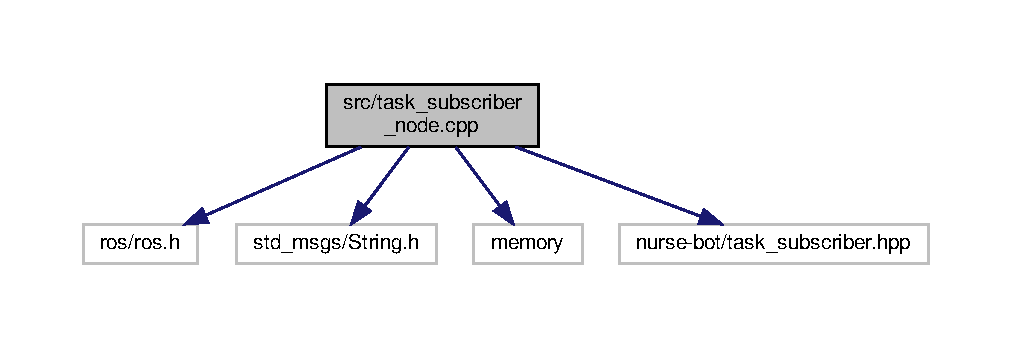
\includegraphics[width=350pt]{task__subscriber__node_8cpp__incl}
\end{center}
\end{figure}
\subsection*{Functions}
\begin{DoxyCompactItemize}
\item 
\mbox{\Hypertarget{task__subscriber__node_8cpp_a3c04138a5bfe5d72780bb7e82a18e627}\label{task__subscriber__node_8cpp_a3c04138a5bfe5d72780bb7e82a18e627}} 
int {\bfseries main} (int argc, char $\ast$$\ast$argv)
\end{DoxyCompactItemize}


\subsection{Detailed Description}
R\+OS node to spawn the subscriber of the task topic. 

M\+IT License

Copyright (c) 2021 Sakshi Kakde, Siddharth Telang, Anubhav Paras

Permission is hereby granted, free of charge, to any person obtaining a copy of this software and associated documentation files (the \char`\"{}\+Software\char`\"{}), to deal in the Software without restriction, including without limitation the rights to use, copy, modify, merge, publish, distribute, sublicense, and/or sell copies of the Software, and to permit persons to whom the Software is furnished to do so, subject to the following conditions\+:

The above copyright notice and this permission notice shall be included in all copies or substantial portions of the Software.

T\+HE S\+O\+F\+T\+W\+A\+RE IS P\+R\+O\+V\+I\+D\+ED \char`\"{}\+A\+S I\+S\char`\"{}, W\+I\+T\+H\+O\+UT W\+A\+R\+R\+A\+N\+TY OF A\+NY K\+I\+ND, E\+X\+P\+R\+E\+SS OR I\+M\+P\+L\+I\+ED, I\+N\+C\+L\+U\+D\+I\+NG B\+UT N\+OT L\+I\+M\+I\+T\+ED TO T\+HE W\+A\+R\+R\+A\+N\+T\+I\+ES OF M\+E\+R\+C\+H\+A\+N\+T\+A\+B\+I\+L\+I\+TY, F\+I\+T\+N\+E\+SS F\+OR A P\+A\+R\+T\+I\+C\+U\+L\+AR P\+U\+R\+P\+O\+SE A\+ND N\+O\+N\+I\+N\+F\+R\+I\+N\+G\+E\+M\+E\+NT. IN NO E\+V\+E\+NT S\+H\+A\+LL T\+HE A\+U\+T\+H\+O\+RS OR C\+O\+P\+Y\+R\+I\+G\+HT H\+O\+L\+D\+E\+RS BE L\+I\+A\+B\+LE F\+OR A\+NY C\+L\+A\+IM, D\+A\+M\+A\+G\+ES OR O\+T\+H\+ER L\+I\+A\+B\+I\+L\+I\+TY, W\+H\+E\+T\+H\+ER IN AN A\+C\+T\+I\+ON OF C\+O\+N\+T\+R\+A\+CT, T\+O\+RT OR O\+T\+H\+E\+R\+W\+I\+SE, A\+R\+I\+S\+I\+NG F\+R\+OM, O\+UT OF OR IN C\+O\+N\+N\+E\+C\+T\+I\+ON W\+I\+TH T\+HE S\+O\+F\+T\+W\+A\+RE OR T\+HE U\+SE OR O\+T\+H\+ER D\+E\+A\+L\+I\+N\+GS IN T\+HE S\+O\+F\+T\+W\+A\+RE.

\begin{DoxyAuthor}{Author}
Sakshi Kakde (\href{mailto:sakshi@umd.edu}{\tt sakshi@umd.\+edu}) 

Siddharth Telang (\href{mailto:stelang@umd.edu}{\tt stelang@umd.\+edu}) 

Anubhav Paras (\href{mailto:anubhavp@umd.edu}{\tt anubhavp@umd.\+edu}) 
\end{DoxyAuthor}
\begin{DoxyVersion}{Version}
0.\+1 
\end{DoxyVersion}
\begin{DoxyDate}{Date}
2021-\/11-\/27
\end{DoxyDate}
\begin{DoxyCopyright}{Copyright}
Copyright (c) 2021 
\end{DoxyCopyright}

\hypertarget{user__interface__node_8cpp}{}\section{src/user\+\_\+interface\+\_\+node.cpp File Reference}
\label{user__interface__node_8cpp}\index{src/user\+\_\+interface\+\_\+node.\+cpp@{src/user\+\_\+interface\+\_\+node.\+cpp}}


R\+OS node for to spawn user interface and publish messages.  


{\ttfamily \#include $<$ros/ros.\+h$>$}\newline
{\ttfamily \#include $<$nurse\+\_\+bot/\+Task.\+h$>$}\newline
{\ttfamily \#include $<$iostream$>$}\newline
{\ttfamily \#include $<$memory$>$}\newline
{\ttfamily \#include $<$sstream$>$}\newline
{\ttfamily \#include $<$nurse-\/bot/task\+\_\+publisher.\+hpp$>$}\newline
Include dependency graph for user\+\_\+interface\+\_\+node.\+cpp\+:
\nopagebreak
\begin{figure}[H]
\begin{center}
\leavevmode
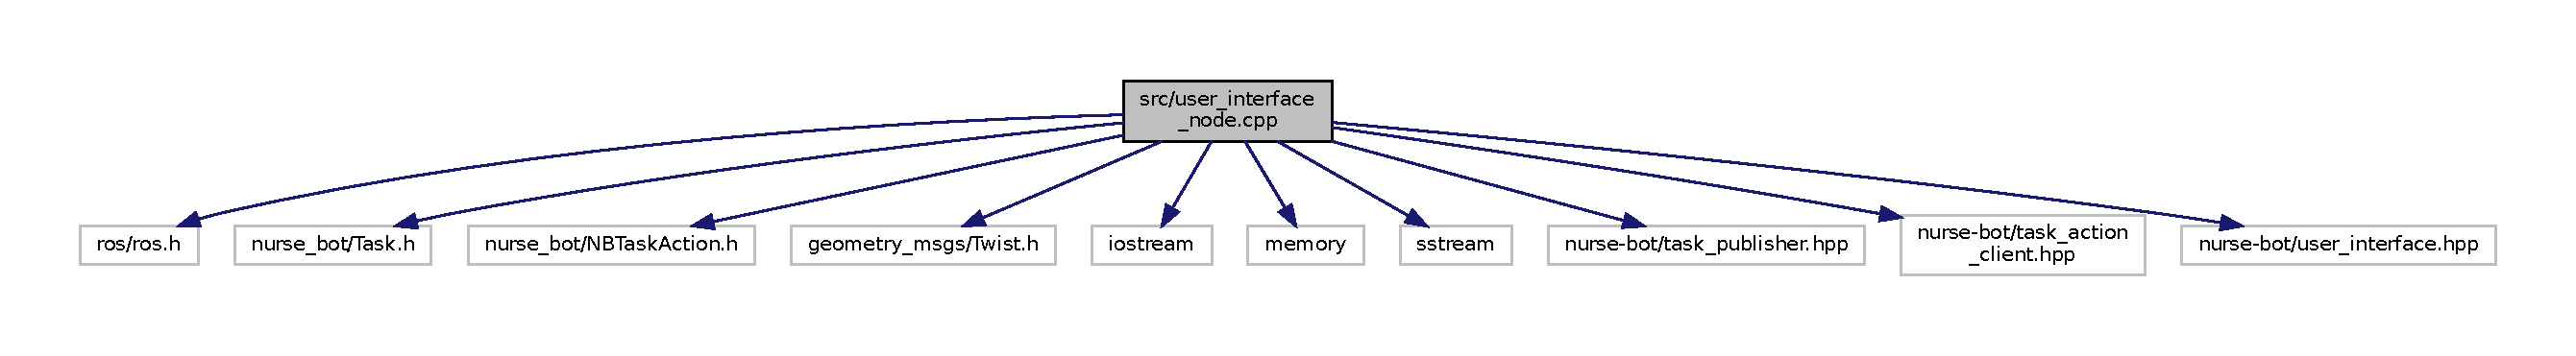
\includegraphics[width=350pt]{user__interface__node_8cpp__incl}
\end{center}
\end{figure}
\subsection*{Functions}
\begin{DoxyCompactItemize}
\item 
\mbox{\Hypertarget{user__interface__node_8cpp_a3c04138a5bfe5d72780bb7e82a18e627}\label{user__interface__node_8cpp_a3c04138a5bfe5d72780bb7e82a18e627}} 
int {\bfseries main} (int argc, char $\ast$$\ast$argv)
\end{DoxyCompactItemize}


\subsection{Detailed Description}
R\+OS node for to spawn user interface and publish messages. 

M\+IT License

Copyright (c) 2021 Sakshi Kakde, Siddharth Telang, Anubhav Paras

Permission is hereby granted, free of charge, to any person obtaining a copy of this software and associated documentation files (the \char`\"{}\+Software\char`\"{}), to deal in the Software without restriction, including without limitation the rights to use, copy, modify, merge, publish, distribute, sublicense, and/or sell copies of the Software, and to permit persons to whom the Software is furnished to do so, subject to the following conditions\+:

The above copyright notice and this permission notice shall be included in all copies or substantial portions of the Software.

T\+HE S\+O\+F\+T\+W\+A\+RE IS P\+R\+O\+V\+I\+D\+ED \char`\"{}\+A\+S I\+S\char`\"{}, W\+I\+T\+H\+O\+UT W\+A\+R\+R\+A\+N\+TY OF A\+NY K\+I\+ND, E\+X\+P\+R\+E\+SS OR I\+M\+P\+L\+I\+ED, I\+N\+C\+L\+U\+D\+I\+NG B\+UT N\+OT L\+I\+M\+I\+T\+ED TO T\+HE W\+A\+R\+R\+A\+N\+T\+I\+ES OF M\+E\+R\+C\+H\+A\+N\+T\+A\+B\+I\+L\+I\+TY, F\+I\+T\+N\+E\+SS F\+OR A P\+A\+R\+T\+I\+C\+U\+L\+AR P\+U\+R\+P\+O\+SE A\+ND N\+O\+N\+I\+N\+F\+R\+I\+N\+G\+E\+M\+E\+NT. IN NO E\+V\+E\+NT S\+H\+A\+LL T\+HE A\+U\+T\+H\+O\+RS OR C\+O\+P\+Y\+R\+I\+G\+HT H\+O\+L\+D\+E\+RS BE L\+I\+A\+B\+LE F\+OR A\+NY C\+L\+A\+IM, D\+A\+M\+A\+G\+ES OR O\+T\+H\+ER L\+I\+A\+B\+I\+L\+I\+TY, W\+H\+E\+T\+H\+ER IN AN A\+C\+T\+I\+ON OF C\+O\+N\+T\+R\+A\+CT, T\+O\+RT OR O\+T\+H\+E\+R\+W\+I\+SE, A\+R\+I\+S\+I\+NG F\+R\+OM, O\+UT OF OR IN C\+O\+N\+N\+E\+C\+T\+I\+ON W\+I\+TH T\+HE S\+O\+F\+T\+W\+A\+RE OR T\+HE U\+SE OR O\+T\+H\+ER D\+E\+A\+L\+I\+N\+GS IN T\+HE S\+O\+F\+T\+W\+A\+RE.

\begin{DoxyAuthor}{Author}
Sakshi Kakde (\href{mailto:sakshi@umd.edu}{\tt sakshi@umd.\+edu}) 

Siddharth Telang (\href{mailto:stelang@umd.edu}{\tt stelang@umd.\+edu}) 

Anubhav Paras (\href{mailto:anubhavp@umd.edu}{\tt anubhavp@umd.\+edu}) 
\end{DoxyAuthor}
\begin{DoxyVersion}{Version}
0.\+1 
\end{DoxyVersion}
\begin{DoxyDate}{Date}
2021-\/11-\/27
\end{DoxyDate}
\begin{DoxyCopyright}{Copyright}
Copyright (c) 2021 
\end{DoxyCopyright}

\hypertarget{main_8cpp}{}\section{test/main.cpp File Reference}
\label{main_8cpp}\index{test/main.\+cpp@{test/main.\+cpp}}


main for controller tests  


{\ttfamily \#include $<$ros/ros.\+h$>$}\newline
{\ttfamily \#include $<$gtest/gtest.\+h$>$}\newline
{\ttfamily \#include $<$atomic$>$}\newline
{\ttfamily \#include $<$thread$>$}\newline
{\ttfamily \#include $<$chrono$>$}\newline
Include dependency graph for main.\+cpp\+:
\nopagebreak
\begin{figure}[H]
\begin{center}
\leavevmode
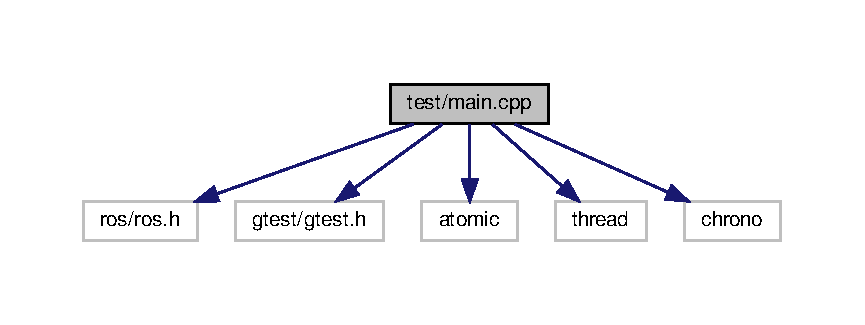
\includegraphics[width=350pt]{main_8cpp__incl}
\end{center}
\end{figure}
\subsection*{Functions}
\begin{DoxyCompactItemize}
\item 
\mbox{\Hypertarget{main_8cpp_a3c04138a5bfe5d72780bb7e82a18e627}\label{main_8cpp_a3c04138a5bfe5d72780bb7e82a18e627}} 
int {\bfseries main} (int argc, char $\ast$$\ast$argv)
\end{DoxyCompactItemize}


\subsection{Detailed Description}
main for controller tests 

Definitions of Map\+Navigator class.

M\+IT License

Copyright (c) 2021 Sakshi Kakde, Siddharth Telang, Anubhav Paras

Permission is hereby granted, free of charge, to any person obtaining a copy of this software and associated documentation files (the \char`\"{}\+Software\char`\"{}), to deal in the Software without restriction, including without limitation the rights to use, copy, modify, merge, publish, distribute, sublicense, and/or sell copies of the Software, and to permit persons to whom the Software is furnished to do so, subject to the following conditions\+:

The above copyright notice and this permission notice shall be included in all copies or substantial portions of the Software.

T\+HE S\+O\+F\+T\+W\+A\+RE IS P\+R\+O\+V\+I\+D\+ED \char`\"{}\+A\+S I\+S\char`\"{}, W\+I\+T\+H\+O\+UT W\+A\+R\+R\+A\+N\+TY OF A\+NY K\+I\+ND, E\+X\+P\+R\+E\+SS OR I\+M\+P\+L\+I\+ED, I\+N\+C\+L\+U\+D\+I\+NG B\+UT N\+OT L\+I\+M\+I\+T\+ED TO T\+HE W\+A\+R\+R\+A\+N\+T\+I\+ES OF M\+E\+R\+C\+H\+A\+N\+T\+A\+B\+I\+L\+I\+TY, F\+I\+T\+N\+E\+SS F\+OR A P\+A\+R\+T\+I\+C\+U\+L\+AR P\+U\+R\+P\+O\+SE A\+ND N\+O\+N\+I\+N\+F\+R\+I\+N\+G\+E\+M\+E\+NT. IN NO E\+V\+E\+NT S\+H\+A\+LL T\+HE A\+U\+T\+H\+O\+RS OR C\+O\+P\+Y\+R\+I\+G\+HT H\+O\+L\+D\+E\+RS BE L\+I\+A\+B\+LE F\+OR A\+NY C\+L\+A\+IM, D\+A\+M\+A\+G\+ES OR O\+T\+H\+ER L\+I\+A\+B\+I\+L\+I\+TY, W\+H\+E\+T\+H\+ER IN AN A\+C\+T\+I\+ON OF C\+O\+N\+T\+R\+A\+CT, T\+O\+RT OR O\+T\+H\+E\+R\+W\+I\+SE, A\+R\+I\+S\+I\+NG F\+R\+OM, O\+UT OF OR IN C\+O\+N\+N\+E\+C\+T\+I\+ON W\+I\+TH T\+HE S\+O\+F\+T\+W\+A\+RE OR T\+HE U\+SE OR O\+T\+H\+ER D\+E\+A\+L\+I\+N\+GS IN T\+HE S\+O\+F\+T\+W\+A\+RE.

\begin{DoxyAuthor}{Author}
Sakshi Kakde (\href{mailto:sakshi@umd.edu}{\tt sakshi@umd.\+edu}) 

Siddharth Telang (\href{mailto:stelang@umd.edu}{\tt stelang@umd.\+edu}) 

Anubhav Paras (\href{mailto:anubhavp@umd.edu}{\tt anubhavp@umd.\+edu}) 
\end{DoxyAuthor}
\begin{DoxyVersion}{Version}
0.\+1 
\end{DoxyVersion}
\begin{DoxyDate}{Date}
2021-\/11-\/27
\end{DoxyDate}
\begin{DoxyCopyright}{Copyright}
Copyright (c) 2021 
\end{DoxyCopyright}

\hypertarget{test__map__navigator_8cpp}{}\doxysection{test/test\+\_\+map\+\_\+navigator.cpp File Reference}
\label{test__map__navigator_8cpp}\index{test/test\_map\_navigator.cpp@{test/test\_map\_navigator.cpp}}


Testing of Map\+Navigator class.  


{\ttfamily \#include $<$gtest/gtest.\+h$>$}\newline
{\ttfamily \#include $<$gmock/gmock.\+h$>$}\newline
{\ttfamily \#include $<$memory$>$}\newline
{\ttfamily \#include $<$nurse-\/bot/mock/movebaseaction\+\_\+wrapper\+\_\+mock.\+hpp$>$}\newline
{\ttfamily \#include $<$nurse-\/bot/pose.\+hpp$>$}\newline
{\ttfamily \#include $<$nurse-\/bot/map\+\_\+navigator.\+hpp$>$}\newline
Include dependency graph for test\+\_\+map\+\_\+navigator.\+cpp\+:
\nopagebreak
\begin{figure}[H]
\begin{center}
\leavevmode
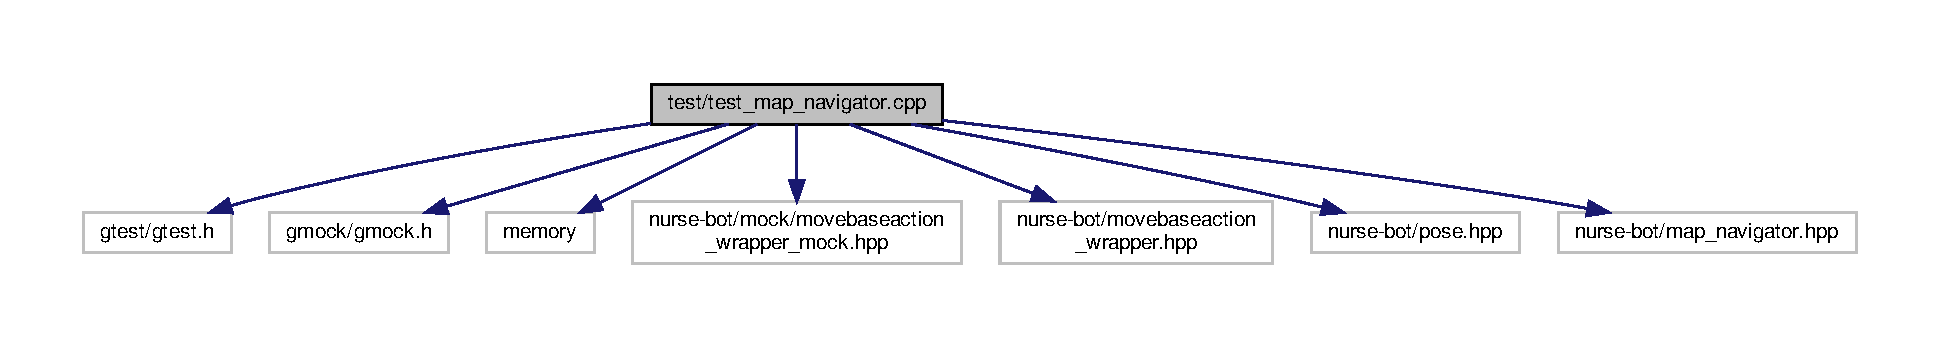
\includegraphics[width=350pt]{test__map__navigator_8cpp__incl}
\end{center}
\end{figure}
\doxysubsection*{Functions}
\begin{DoxyCompactItemize}
\item 
\mbox{\Hypertarget{test__map__navigator_8cpp_a48049295df925a849220878fe4d596d8}\label{test__map__navigator_8cpp_a48049295df925a849220878fe4d596d8}} 
{\bfseries T\+E\+ST} (Map\+Navigator\+Test, test\+Navigate\+Method)
\end{DoxyCompactItemize}


\doxysubsection{Detailed Description}
Testing of Map\+Navigator class. 

M\+IT License

Copyright (c) 2021 Sakshi Kakde, Siddharth Telang, Anubhav Paras

Permission is hereby granted, free of charge, to any person obtaining a copy of this software and associated documentation files (the \char`\"{}\+Software\char`\"{}), to deal in the Software without restriction, including without limitation the rights to use, copy, modify, merge, publish, distribute, sublicense, and/or sell copies of the Software, and to permit persons to whom the Software is furnished to do so, subject to the following conditions\+:

The above copyright notice and this permission notice shall be included in all copies or substantial portions of the Software.

T\+HE S\+O\+F\+T\+W\+A\+RE IS P\+R\+O\+V\+I\+D\+ED \char`\"{}\+A\+S I\+S\char`\"{}, W\+I\+T\+H\+O\+UT W\+A\+R\+R\+A\+N\+TY OF A\+NY K\+I\+ND, E\+X\+P\+R\+E\+SS OR I\+M\+P\+L\+I\+ED, I\+N\+C\+L\+U\+D\+I\+NG B\+UT N\+OT L\+I\+M\+I\+T\+ED TO T\+HE W\+A\+R\+R\+A\+N\+T\+I\+ES OF M\+E\+R\+C\+H\+A\+N\+T\+A\+B\+I\+L\+I\+TY, F\+I\+T\+N\+E\+SS F\+OR A P\+A\+R\+T\+I\+C\+U\+L\+AR P\+U\+R\+P\+O\+SE A\+ND N\+O\+N\+I\+N\+F\+R\+I\+N\+G\+E\+M\+E\+NT. IN NO E\+V\+E\+NT S\+H\+A\+LL T\+HE A\+U\+T\+H\+O\+RS OR C\+O\+P\+Y\+R\+I\+G\+HT H\+O\+L\+D\+E\+RS BE L\+I\+A\+B\+LE F\+OR A\+NY C\+L\+A\+IM, D\+A\+M\+A\+G\+ES OR O\+T\+H\+ER L\+I\+A\+B\+I\+L\+I\+TY, W\+H\+E\+T\+H\+ER IN AN A\+C\+T\+I\+ON OF C\+O\+N\+T\+R\+A\+CT, T\+O\+RT OR O\+T\+H\+E\+R\+W\+I\+SE, A\+R\+I\+S\+I\+NG F\+R\+OM, O\+UT OF OR IN C\+O\+N\+N\+E\+C\+T\+I\+ON W\+I\+TH T\+HE S\+O\+F\+T\+W\+A\+RE OR T\+HE U\+SE OR O\+T\+H\+ER D\+E\+A\+L\+I\+N\+GS IN T\+HE S\+O\+F\+T\+W\+A\+RE.

\begin{DoxyAuthor}{Author}
Sakshi Kakde (\href{mailto:sakshi@umd.edu}{\texttt{ sakshi@umd.\+edu}}) 

Siddharth Telang (\href{mailto:stelang@umd.edu}{\texttt{ stelang@umd.\+edu}}) 

Anubhav Paras (\href{mailto:anubhavp@umd.edu}{\texttt{ anubhavp@umd.\+edu}}) 
\end{DoxyAuthor}
\begin{DoxyVersion}{Version}
0.\+1 
\end{DoxyVersion}
\begin{DoxyDate}{Date}
2021-\/11-\/27
\end{DoxyDate}
\begin{DoxyCopyright}{Copyright}
Copyright (c) 2021 
\end{DoxyCopyright}

\hypertarget{test__movebaseaction__wrapper_8cpp}{}\doxysection{test/test\+\_\+movebaseaction\+\_\+wrapper.cpp File Reference}
\label{test__movebaseaction__wrapper_8cpp}\index{test/test\_movebaseaction\_wrapper.cpp@{test/test\_movebaseaction\_wrapper.cpp}}


Testing of Move\+Base\+Action\+Wrapper class.  


{\ttfamily \#include $<$gtest/gtest.\+h$>$}\newline
{\ttfamily \#include $<$gmock/gmock.\+h$>$}\newline
{\ttfamily \#include $<$memory$>$}\newline
{\ttfamily \#include $<$string$>$}\newline
{\ttfamily \#include $<$nurse-\/bot/mock/movebaseaction\+\_\+wrapper\+\_\+mock.\+hpp$>$}\newline
{\ttfamily \#include $<$nurse-\/bot/pose.\+hpp$>$}\newline
{\ttfamily \#include $<$nurse-\/bot/movebaseaction\+\_\+wrapper.\+hpp$>$}\newline
Include dependency graph for test\+\_\+movebaseaction\+\_\+wrapper.\+cpp\+:
\nopagebreak
\begin{figure}[H]
\begin{center}
\leavevmode
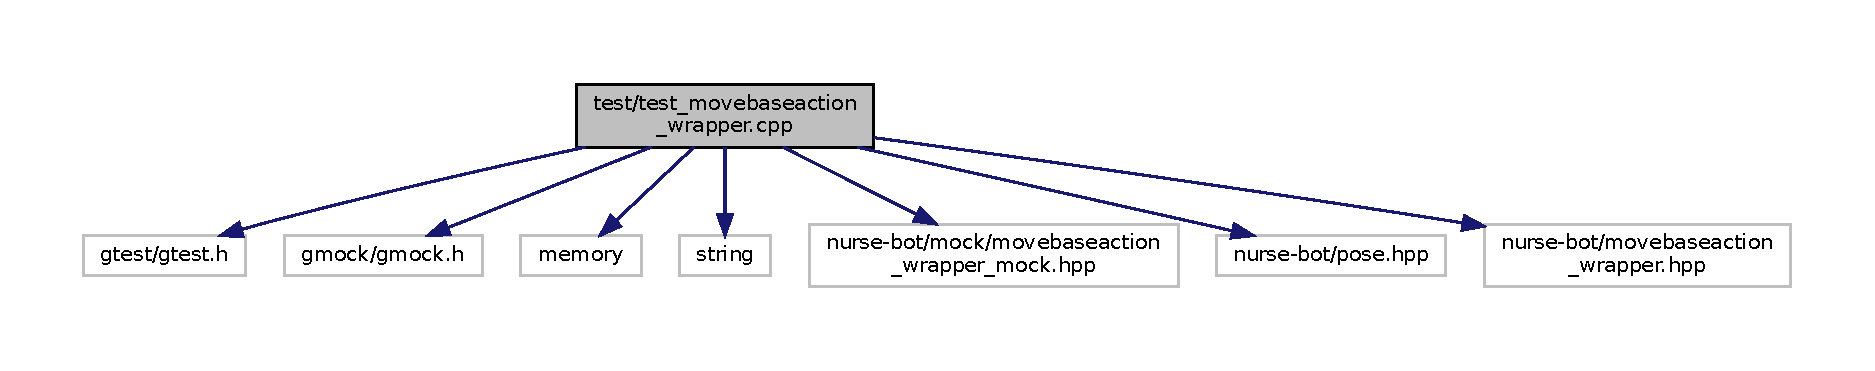
\includegraphics[width=350pt]{test__movebaseaction__wrapper_8cpp__incl}
\end{center}
\end{figure}
\doxysubsection*{Functions}
\begin{DoxyCompactItemize}
\item 
\mbox{\Hypertarget{test__movebaseaction__wrapper_8cpp_a315cebdb4e4a5ef709bc45da76bc3e61}\label{test__movebaseaction__wrapper_8cpp_a315cebdb4e4a5ef709bc45da76bc3e61}} 
{\bfseries T\+E\+ST} (Move\+Base\+Action\+Wrapper\+Test, test\+Sendgoal)
\end{DoxyCompactItemize}


\doxysubsection{Detailed Description}
Testing of Move\+Base\+Action\+Wrapper class. 

M\+IT License

Copyright (c) 2021 Sakshi Kakde, Siddharth Telang, Anubhav Paras

Permission is hereby granted, free of charge, to any person obtaining a copy of this software and associated documentation files (the \char`\"{}\+Software\char`\"{}), to deal in the Software without restriction, including without limitation the rights to use, copy, modify, merge, publish, distribute, sublicense, and/or sell copies of the Software, and to permit persons to whom the Software is furnished to do so, subject to the following conditions\+:

The above copyright notice and this permission notice shall be included in all copies or substantial portions of the Software.

T\+HE S\+O\+F\+T\+W\+A\+RE IS P\+R\+O\+V\+I\+D\+ED \char`\"{}\+A\+S I\+S\char`\"{}, W\+I\+T\+H\+O\+UT W\+A\+R\+R\+A\+N\+TY OF A\+NY K\+I\+ND, E\+X\+P\+R\+E\+SS OR I\+M\+P\+L\+I\+ED, I\+N\+C\+L\+U\+D\+I\+NG B\+UT N\+OT L\+I\+M\+I\+T\+ED TO T\+HE W\+A\+R\+R\+A\+N\+T\+I\+ES OF M\+E\+R\+C\+H\+A\+N\+T\+A\+B\+I\+L\+I\+TY, F\+I\+T\+N\+E\+SS F\+OR A P\+A\+R\+T\+I\+C\+U\+L\+AR P\+U\+R\+P\+O\+SE A\+ND N\+O\+N\+I\+N\+F\+R\+I\+N\+G\+E\+M\+E\+NT. IN NO E\+V\+E\+NT S\+H\+A\+LL T\+HE A\+U\+T\+H\+O\+RS OR C\+O\+P\+Y\+R\+I\+G\+HT H\+O\+L\+D\+E\+RS BE L\+I\+A\+B\+LE F\+OR A\+NY C\+L\+A\+IM, D\+A\+M\+A\+G\+ES OR O\+T\+H\+ER L\+I\+A\+B\+I\+L\+I\+TY, W\+H\+E\+T\+H\+ER IN AN A\+C\+T\+I\+ON OF C\+O\+N\+T\+R\+A\+CT, T\+O\+RT OR O\+T\+H\+E\+R\+W\+I\+SE, A\+R\+I\+S\+I\+NG F\+R\+OM, O\+UT OF OR IN C\+O\+N\+N\+E\+C\+T\+I\+ON W\+I\+TH T\+HE S\+O\+F\+T\+W\+A\+RE OR T\+HE U\+SE OR O\+T\+H\+ER D\+E\+A\+L\+I\+N\+GS IN T\+HE S\+O\+F\+T\+W\+A\+RE.

\begin{DoxyAuthor}{Author}
Sakshi Kakde (\href{mailto:sakshi@umd.edu}{\texttt{ sakshi@umd.\+edu}}) 

Siddharth Telang (\href{mailto:stelang@umd.edu}{\texttt{ stelang@umd.\+edu}}) 

Anubhav Paras (\href{mailto:anubhavp@umd.edu}{\texttt{ anubhavp@umd.\+edu}}) 
\end{DoxyAuthor}
\begin{DoxyVersion}{Version}
0.\+1 
\end{DoxyVersion}
\begin{DoxyDate}{Date}
2021-\/11-\/27
\end{DoxyDate}
\begin{DoxyCopyright}{Copyright}
Copyright (c) 2021 
\end{DoxyCopyright}

\hypertarget{test__task__action_8cpp}{}\section{test/test\+\_\+task\+\_\+action.cpp File Reference}
\label{test__task__action_8cpp}\index{test/test\+\_\+task\+\_\+action.\+cpp@{test/test\+\_\+task\+\_\+action.\+cpp}}


Testing of Guidance\+Task and Delivery\+Task class.  


{\ttfamily \#include $<$gtest/gtest.\+h$>$}\newline
{\ttfamily \#include $<$gmock/gmock.\+h$>$}\newline
{\ttfamily \#include $<$nurse\+\_\+bot/\+Task.\+h$>$}\newline
{\ttfamily \#include $<$memory$>$}\newline
{\ttfamily \#include $<$nurse-\/bot/mock/navigator\+\_\+mock.\+hpp$>$}\newline
{\ttfamily \#include $<$nurse-\/bot/task\+\_\+action.\+hpp$>$}\newline
Include dependency graph for test\+\_\+task\+\_\+action.\+cpp\+:
\nopagebreak
\begin{figure}[H]
\begin{center}
\leavevmode
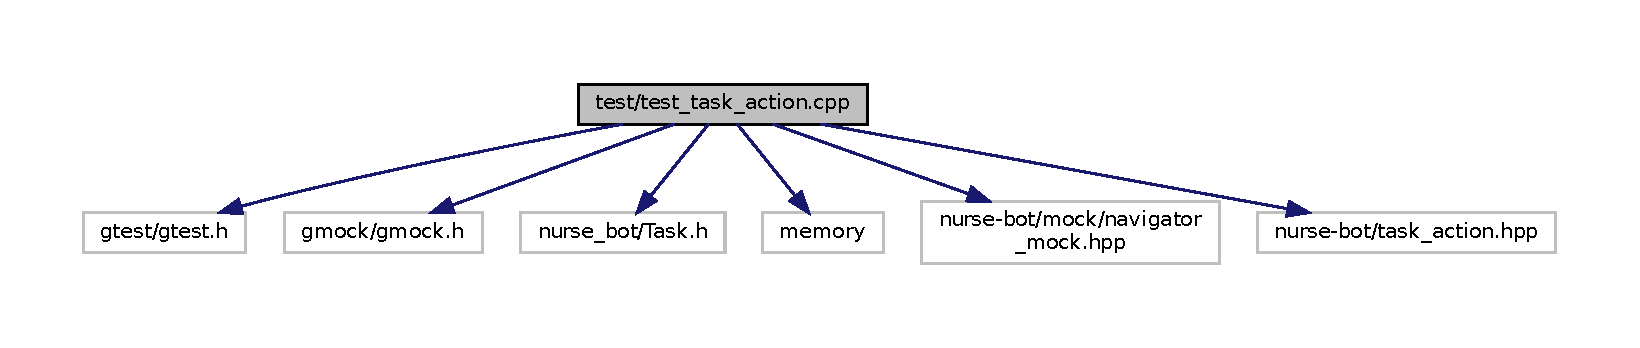
\includegraphics[width=350pt]{test__task__action_8cpp__incl}
\end{center}
\end{figure}
\subsection*{Functions}
\begin{DoxyCompactItemize}
\item 
\mbox{\Hypertarget{test__task__action_8cpp_a84afc1dcc4d8ffdddd0e8404630d430c}\label{test__task__action_8cpp_a84afc1dcc4d8ffdddd0e8404630d430c}} 
{\bfseries T\+E\+ST} (Guidance\+Task\+Test, test\+Perform\+Task\+Method\+\_\+target\+Reached)
\item 
\mbox{\Hypertarget{test__task__action_8cpp_a78e9abca47109d6d0c76eb0897e4dedc}\label{test__task__action_8cpp_a78e9abca47109d6d0c76eb0897e4dedc}} 
{\bfseries T\+E\+ST} (Guidance\+Task\+Test, test\+Perform\+Task\+Method\+\_\+did\+Not\+Reach\+Entity)
\item 
\mbox{\Hypertarget{test__task__action_8cpp_ac4a383b77fe675e9757ae4551544d676}\label{test__task__action_8cpp_ac4a383b77fe675e9757ae4551544d676}} 
{\bfseries T\+E\+ST} (Guidance\+Task\+Test, test\+Perform\+Task\+Method\+\_\+did\+Not\+Reach\+Target)
\item 
\mbox{\Hypertarget{test__task__action_8cpp_a50d46e37adf6a8f9ada720f26ad4a97b}\label{test__task__action_8cpp_a50d46e37adf6a8f9ada720f26ad4a97b}} 
{\bfseries T\+E\+ST} (Delivery\+Task\+Test, test\+Perform\+Task\+Method\+\_\+target\+Reached)
\item 
\mbox{\Hypertarget{test__task__action_8cpp_a740664352cf6190145794169830bdb0b}\label{test__task__action_8cpp_a740664352cf6190145794169830bdb0b}} 
{\bfseries T\+E\+ST} (Delivery\+Task\+Test, test\+Perform\+Task\+Method\+\_\+did\+Not\+Reach\+Entity)
\item 
\mbox{\Hypertarget{test__task__action_8cpp_acb45c3ca7e77a07ac1d1c70217b34243}\label{test__task__action_8cpp_acb45c3ca7e77a07ac1d1c70217b34243}} 
{\bfseries T\+E\+ST} (Delivery\+Task\+Test, test\+Perform\+Task\+Method\+\_\+did\+Not\+Reach\+Target)
\end{DoxyCompactItemize}


\subsection{Detailed Description}
Testing of Guidance\+Task and Delivery\+Task class. 

Testing of Task\+Publisher class.

M\+IT License

Copyright (c) 2021 Sakshi Kakde, Siddharth Telang, Anubhav Paras

Permission is hereby granted, free of charge, to any person obtaining a copy of this software and associated documentation files (the \char`\"{}\+Software\char`\"{}), to deal in the Software without restriction, including without limitation the rights to use, copy, modify, merge, publish, distribute, sublicense, and/or sell copies of the Software, and to permit persons to whom the Software is furnished to do so, subject to the following conditions\+:

The above copyright notice and this permission notice shall be included in all copies or substantial portions of the Software.

T\+HE S\+O\+F\+T\+W\+A\+RE IS P\+R\+O\+V\+I\+D\+ED \char`\"{}\+A\+S I\+S\char`\"{}, W\+I\+T\+H\+O\+UT W\+A\+R\+R\+A\+N\+TY OF A\+NY K\+I\+ND, E\+X\+P\+R\+E\+SS OR I\+M\+P\+L\+I\+ED, I\+N\+C\+L\+U\+D\+I\+NG B\+UT N\+OT L\+I\+M\+I\+T\+ED TO T\+HE W\+A\+R\+R\+A\+N\+T\+I\+ES OF M\+E\+R\+C\+H\+A\+N\+T\+A\+B\+I\+L\+I\+TY, F\+I\+T\+N\+E\+SS F\+OR A P\+A\+R\+T\+I\+C\+U\+L\+AR P\+U\+R\+P\+O\+SE A\+ND N\+O\+N\+I\+N\+F\+R\+I\+N\+G\+E\+M\+E\+NT. IN NO E\+V\+E\+NT S\+H\+A\+LL T\+HE A\+U\+T\+H\+O\+RS OR C\+O\+P\+Y\+R\+I\+G\+HT H\+O\+L\+D\+E\+RS BE L\+I\+A\+B\+LE F\+OR A\+NY C\+L\+A\+IM, D\+A\+M\+A\+G\+ES OR O\+T\+H\+ER L\+I\+A\+B\+I\+L\+I\+TY, W\+H\+E\+T\+H\+ER IN AN A\+C\+T\+I\+ON OF C\+O\+N\+T\+R\+A\+CT, T\+O\+RT OR O\+T\+H\+E\+R\+W\+I\+SE, A\+R\+I\+S\+I\+NG F\+R\+OM, O\+UT OF OR IN C\+O\+N\+N\+E\+C\+T\+I\+ON W\+I\+TH T\+HE S\+O\+F\+T\+W\+A\+RE OR T\+HE U\+SE OR O\+T\+H\+ER D\+E\+A\+L\+I\+N\+GS IN T\+HE S\+O\+F\+T\+W\+A\+RE.

\begin{DoxyAuthor}{Author}
Sakshi Kakde (\href{mailto:sakshi@umd.edu}{\tt sakshi@umd.\+edu}) 

Siddharth Telang (\href{mailto:stelang@umd.edu}{\tt stelang@umd.\+edu}) 

Anubhav Paras (\href{mailto:anubhavp@umd.edu}{\tt anubhavp@umd.\+edu}) 
\end{DoxyAuthor}
\begin{DoxyVersion}{Version}
0.\+1 
\end{DoxyVersion}
\begin{DoxyDate}{Date}
2021-\/11-\/27
\end{DoxyDate}
\begin{DoxyCopyright}{Copyright}
Copyright (c) 2021 
\end{DoxyCopyright}

%--- End generated contents ---

% Index
\backmatter
\newpage
\phantomsection
\clearemptydoublepage
\addcontentsline{toc}{chapter}{Index}
\printindex

\end{document}
